\lecture{LECTURE: Coursework \& Entity Relationship Diagrams}{20-10-22}{13:00}{Mark}{RB LT1}

\section*{Coursework}
\begin{link}{Coursework}
    The coursework is now available on Moodle, within Assessment and Support Materials.
\end{link}
The deadline for the coursework isn't until February.

It is recommended to submit the files to Moodle well in advance of the deadline because there is a chance there will be a technical issue with Moodle when the deadline is, no extenuating circumstances will be given if this is the case.

The Entity Relationship Diagram submitted must be produced digitally, hand drawn diagrams will gain 0 credits.

Mark uses Mocakroo and Lucid Charts for generating dummy data and drawing ERDs respectively. This is what works well for him, there are other platforms available for both, with more information in the Coursework document.

\section*{Entity Relationship Diagrams}
Entity Relationship Diagrams (ERDs) are diagrams which show how entities are related, down to the detail of what the attributes are and how they relate to each other as well. 

\subsection*{Business Rules}
When designing databases, business rules will be taken into consideration.
\define{Business Ruls}{A statement that defines how a company does stuff or how stuff works within a company.}
We can use business rules to help guide us on how to design databases.

\subsection*{Relationship Links}
We will be using Crows Foot Notation, there are a number of other types of notation however we won't look at any of these.
\begin{figure}[H]
    \centering
    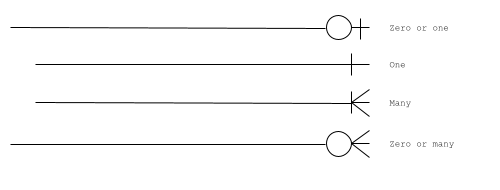
\includegraphics[width=0.8\textwidth]{assets/relationship-links.png}
    \caption{Crow's feet notation}
\end{figure}
When designing entities, it is important to name them in the singular, for example \verb|pig| not \verb|pigs|, and to use underscore notation where multiple words comprise the entity name, not camel notation.

Many-to-many relationships are not permitted. We will return to this in a future lecture.

\section*{Constraints}
\define{Constraint}{A rule that protects your data or enforces certain behaviour.}

For example, a constraint may be set to be \verb|NOT NULL|, this would ensure that whenever a row of data is inserted into a table, that attribute would have to contain data.

Keys are constraints. The primary key is automatically set to be \verb|NOT NULL|, we do not have to specify that when creating a table. We could use a default constraint, to specify the the time that a record was entered into a table. 

Check constraints can be used to validate data as it is entered, for example a price must contain two decimal places. Check may be needed as part of the coursework.